\documentclass[a4paper, 10pt]{article}
\usepackage{float}
\usepackage{graphicx}
\usepackage{subcaption}
\usepackage{hyperref}

\begin{document}

\section*{Metrics}
This is the list of questions which will be attached to the funding process from Asha. It is a result of combining the most useful data from the various papers in addition to being practical about the data that can be collected by a project steward. Ideally we would like to collect more data but at present, this is not possible. It is something to work for in the future as the collection of this kind of data becomes easier. 

\begin{enumerate}

\item Employment status of graduates (by type - full time, casual, self-employed, unemployed, further education)

\item Employment by sector (agricultural, manufacturing, services, other)

\item Student : Teacher ratio (by course)

\item No. of droputs / completion rate (by course)

\item Demographics of participants (by course)
	\begin{itemize}
	\item Age (below 20 / over 20)
	\item Gender (male / female)
	\item Marital Status (single / divorced / married)
	\end{itemize}

\item Total number of seats offered

\item Number of unfilled seats

\end{enumerate}

\section*{Theoretical Framework}

Having collected the data above, we now need to compare a program to other similar ones; this gives an indication of which are more successful (and why) such that the lessons learnt can be applied to other programs. This process is made significantly easier if we standardise the procedure. To this end, most projects follow this 4 part approach \textsuperscript{[2]}:

\begin{itemize}
\item Inputs - the resources invested in a program (time, cost etc.)
\item Activities - the steps taken as part of the program (training, teaching etc.)
\item Outputs - these are individual benefits to participants such as a gain in knowledge and/or skills
\item Outcomes - a large-scale, usually measurable, effect as a result of the program
\end{itemize}

\noindent Often, while we can prove correlation between inputs and outputs, the causal link is much harder. To say that a certain outcome occurred because of the program, \textit{and would not have otherwise}, is almost impossible to show. However, by following certain prescribed procedures, we can try and narrow down the effect of non-control variables in a study. Figure~\ref{fig:framework} shows the framework of our approach.

\begin{figure}[h]
	\centering
	\centerline{
		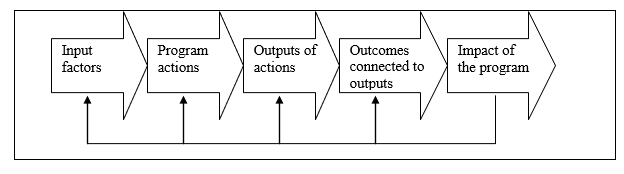
\includegraphics[scale=0.75]{framework.png}
	}
	\caption{Analysis Framework \textsuperscript{[12]}}
    \label{fig:framework}
\end{figure}

\section*{Impact Evaluation}

In an ideal world, the data would be collected in a scientific manner as outlined by REAP (Rural Education Action Program), a self-proclaimed "impact evaluation organisation" that helped tackle China's education, health and nutritional problems \textsuperscript{[6]}. However, considering the current situation in India, this is extremely difficult to organise and implement. The published strategies are something to aim for in the future when conducting an impact evaluation \textsuperscript{[6]}. The highlights are presented here:

\subparagraph*{Randomness}
This is the closest we can come to prove causation as well as correlation. There are two sets of participants, with one group as beneficiaries and the other as a control group. Ideally, this should be the only difference between the two groups such that other random variables affect both groups equally. The group members must also be selected at random, in an unbiased manner to include people of all genders, nationalities, socio-economic backgrounds and education levels. 

\subparagraph*{Relevance}
The impact evaluation must be carried on a program that is realistic and addresses the situation. The input of local councils, governments and organisations is essential - the people who can make a difference must be involved with the evaluation at every stage. 	The aim is not to conduct research or gain a theoretical understanding; it is to make a practical difference on the ground. 

\subparagraph*{Ambitions}
The policy should start small with evaluations carried out at every stage of development. Both the positives and negatives from the smaller pilots should be taken into account before moving on to design the policy with a bigger group. 

\subparagraph*{Continuity}
Impact evaluations are not one-off events; continuous monitoring of a scheme is required to ensure that the highest standards are maintained. In particular, tying further funding to performance is a good incentive to learn from the evaluations and implement the changes suggested.  

\subparagraph*{Communication}
The right data has to be made available to the right people in the right format. As a simple example, policymakers will want a yes/no answer with a short justification as the result of an evaluation. A more scientific audience would require the data collected and the conclusions drawn in more detail so that the work can be independently reviewed. For the general public, a summary of the intervention and its impact suffices. 

\end{document}
